\documentclass[a4paper,11pt]{ltjsarticle}
\usepackage{graphicx}
\usepackage{luatexja-fontspec}
\usepackage{caption}
\usepackage{amsmath,amssymb,bm,braket}
\usepackage[english]{babel}
\usepackage{multicol}
\usepackage{titlesec}
%\usepackage{gnuplot-lua-tikz}
\usepackage[top=20truemm,bottom=20truemm,left=20truemm,right=20truemm]{geometry}
\usepackage{array}
\usepackage{upgreek}
\usepackage{fancyhdr}
\renewcommand{\refname}{}
\usepackage{listings,jvlisting}
\usepackage{tikz}
\usepackage[thmmarks,amsmath]{ntheorem}
\usepackage[version=3]{mhchem}
\usetikzlibrary{external}
\tikzexternalize
\lstset{
  basicstyle={\ttfamily},
  identifierstyle={\small},
  commentstyle={\smallitshape},
  keywordstyle={\small\bfseries},
  ndkeywordstyle={\small},
  stringstyle={\small\ttfamily},
  frame={tb},
  breaklines=true,
  columns=[l]{fullflexible},
  numbers=left,
  xrightmargin=0pt,
  xleftmargin=3pt,
  numberstyle={\scriptsize},
  stepnumber=1,
  numbersep=1pt,
  lineskip=-0.5ex
}
\captionsetup[figure]{format=plain, labelformat=simple, labelsep=quad,labelfont=bf,name={Fig.}}
\captionsetup[table]{format=plain, labelformat=simple, labelsep=quad,labelfont=bf}
\parindent = 0pt
%[BoldFont=HGSMinchoE]{MSMincho}[BoldFont=HiraMinProN-W6]{HiraMinPro-W3}
\titleformat{\section}{\normalfont\fontsize{9}{10}\bfseries\fontspec{Times New Roman}}{\thesection.}{1em}{}
\usepackage[backend=biber,sorting=none,style=numeric,maxnames=99,minnames=1]{biblatex}
\addbibresource{utility/REFERENCES.bib}
\defbibheading{bibliography}[\refname]{%
  \section*{REFERENCES}%
  \vspace{-7pt}  % ここで空白を調整。お好みの値に変更してください。
}
\newfontfamily\subsectionfont{Times New Roman} % サブセクション用フォント
\titleformat{\subsection}
  {\normalfont\large\bfseries} % サブセクションのフォントを指定
  {\thesubsection}{1em}{}
\renewbibmacro{in:}{}
\renewbibmacro*{journal+issuetitle}{%
  \addcomma\space% カンマとスペースを追加
  \usebibmacro{journal}%
  \setunit*{\addspace}%
  \usebibmacro{volume+number+eid}%
  \setunit{\addspace}%
  \printfield{note}%
  \newunit
}
\renewbibmacro*{volume+number+eid}{
  \printfield{volume}%
  \setunit*{\addnbspace}%
  \printfield{number}%
  \setunit{\addcomma\space}%
  \printfield{eid}
}
\DeclareFieldFormat[article]{volume}{\textbf{#1}}
\DeclareFieldFormat[article]{pages}{#1}
\DeclareFieldFormat{journaltitle}{#1}
\usepackage{hyperref}
\renewenvironment{abstract}{\par\noindent}{\par}
%\pagenumbering{gobble}
\usepackage{docmute}
\usepackage{setspace}
\usepackage{titlesec} % 見出しのカスタマイズ用

% セクションのフォーマットをカスタマイズ
\titleformat{\section}
  {} % フォントサイズとスタイル
  {\Large\bfseries\thesection\ \ }               % 番号の前の内容(空白)
  {0em}            % 番号とタイトルの間の間隔
  {\Large\bfseries}


\theoremstyle{plain}
\theoremheaderfont{\normalfont\bfseries}
\theorembodyfont{\itshape}   % 本文を斜体に
\theoremseparator{.}         % タイトルと本文の区切りを「.」に設定
\newtheorem{definition}{Definition}
\begin{document}
\section{Pseudo Three-dimensional Surface Code}{
    \ \ \ In this section, we describe the pseudo three-dimensional Surface Code on the looped pipeline architecture introduced in Section~\ref{looped_pipeline}. First, we describe how computation is performed on multiple 2D Surface Codes in a processor. Then, we extend this concept into a pseudo three-dimensional structure with a periodic cycle in the direction of the third dimension.

    \subsection{Quantum Processor}{
        \ \ \ In fault-tolerant quantum computation, the Surface Code, introduced in Section~\ref{surface_code}, is the most promising error correction code for the calculations required in many quantum algorithms. On the other hand, quantum low-density parity-check codes (qLDPC) are often considered more suitable for quantum memory due to their high encoding rate. However, while a single Surface Code can encode only one logical qubit, it offers many advantages, such as a simple approach for universal logical operations using lattice surgery combined with magic state distillation.

        \ \ \ When designing the processor for computation, we simplify a single Surface Code into a "patch," which features dashed and solid lines. Simply put, a patch represents a logical qubit. In Fig.~\ref{patch}(a), three patches are allocated on the processor, and the corresponding Surface Codes are shown in Fig.~\ref{patch}(b), which are numbered. The rest of the qubits in Fig.~\ref{patch}(b) are unused data qubits for lattice surgery, as introduced in Section~\ref{lattice_surgery}.
        \begin{figure}[h]
            \centering
            \includegraphics[scale=0.20]{figure/patch.eps}
            \vspace{0pt}\caption{}
            \label{patch}
            \vspace{-10pt}
        \end{figure}

        \clearpage

        Using lattice surgery, we can perform logical operations between two patches, three patches, or more. Additionally, we can perform commutative surgery operations in parallel when there exists a route from the control qubit to the target qubit by using unused data qubits in the processor. In this scheme, the efficiency of computation depends on how many parallel operations we can execute, thus requiring careful decision-making regarding the routing of operations. For instance, a certain logical 2-qubit operation between patch 2 and patch 3 is shown in Fig.~\ref{patch_operation}. In this case, we cannot perform a logical operation between patch 1 and patch 2 in parallel.

        \begin{figure}[h]
            \centering
            \includegraphics[scale=0.20]{figure/patch_operation.eps}
            \vspace{0pt}\caption{}
            \label{patch_operation}
            \vspace{-10pt}
        \end{figure}
        
        In Fig.~\ref{qubit_plane}, some logical operations performed in parallel are illustrated with blue routes, while the orange route is prohibited since it intersects with an existing blue route at their intersection.
        \clearpage

        \begin{figure}[h]
            \centering
            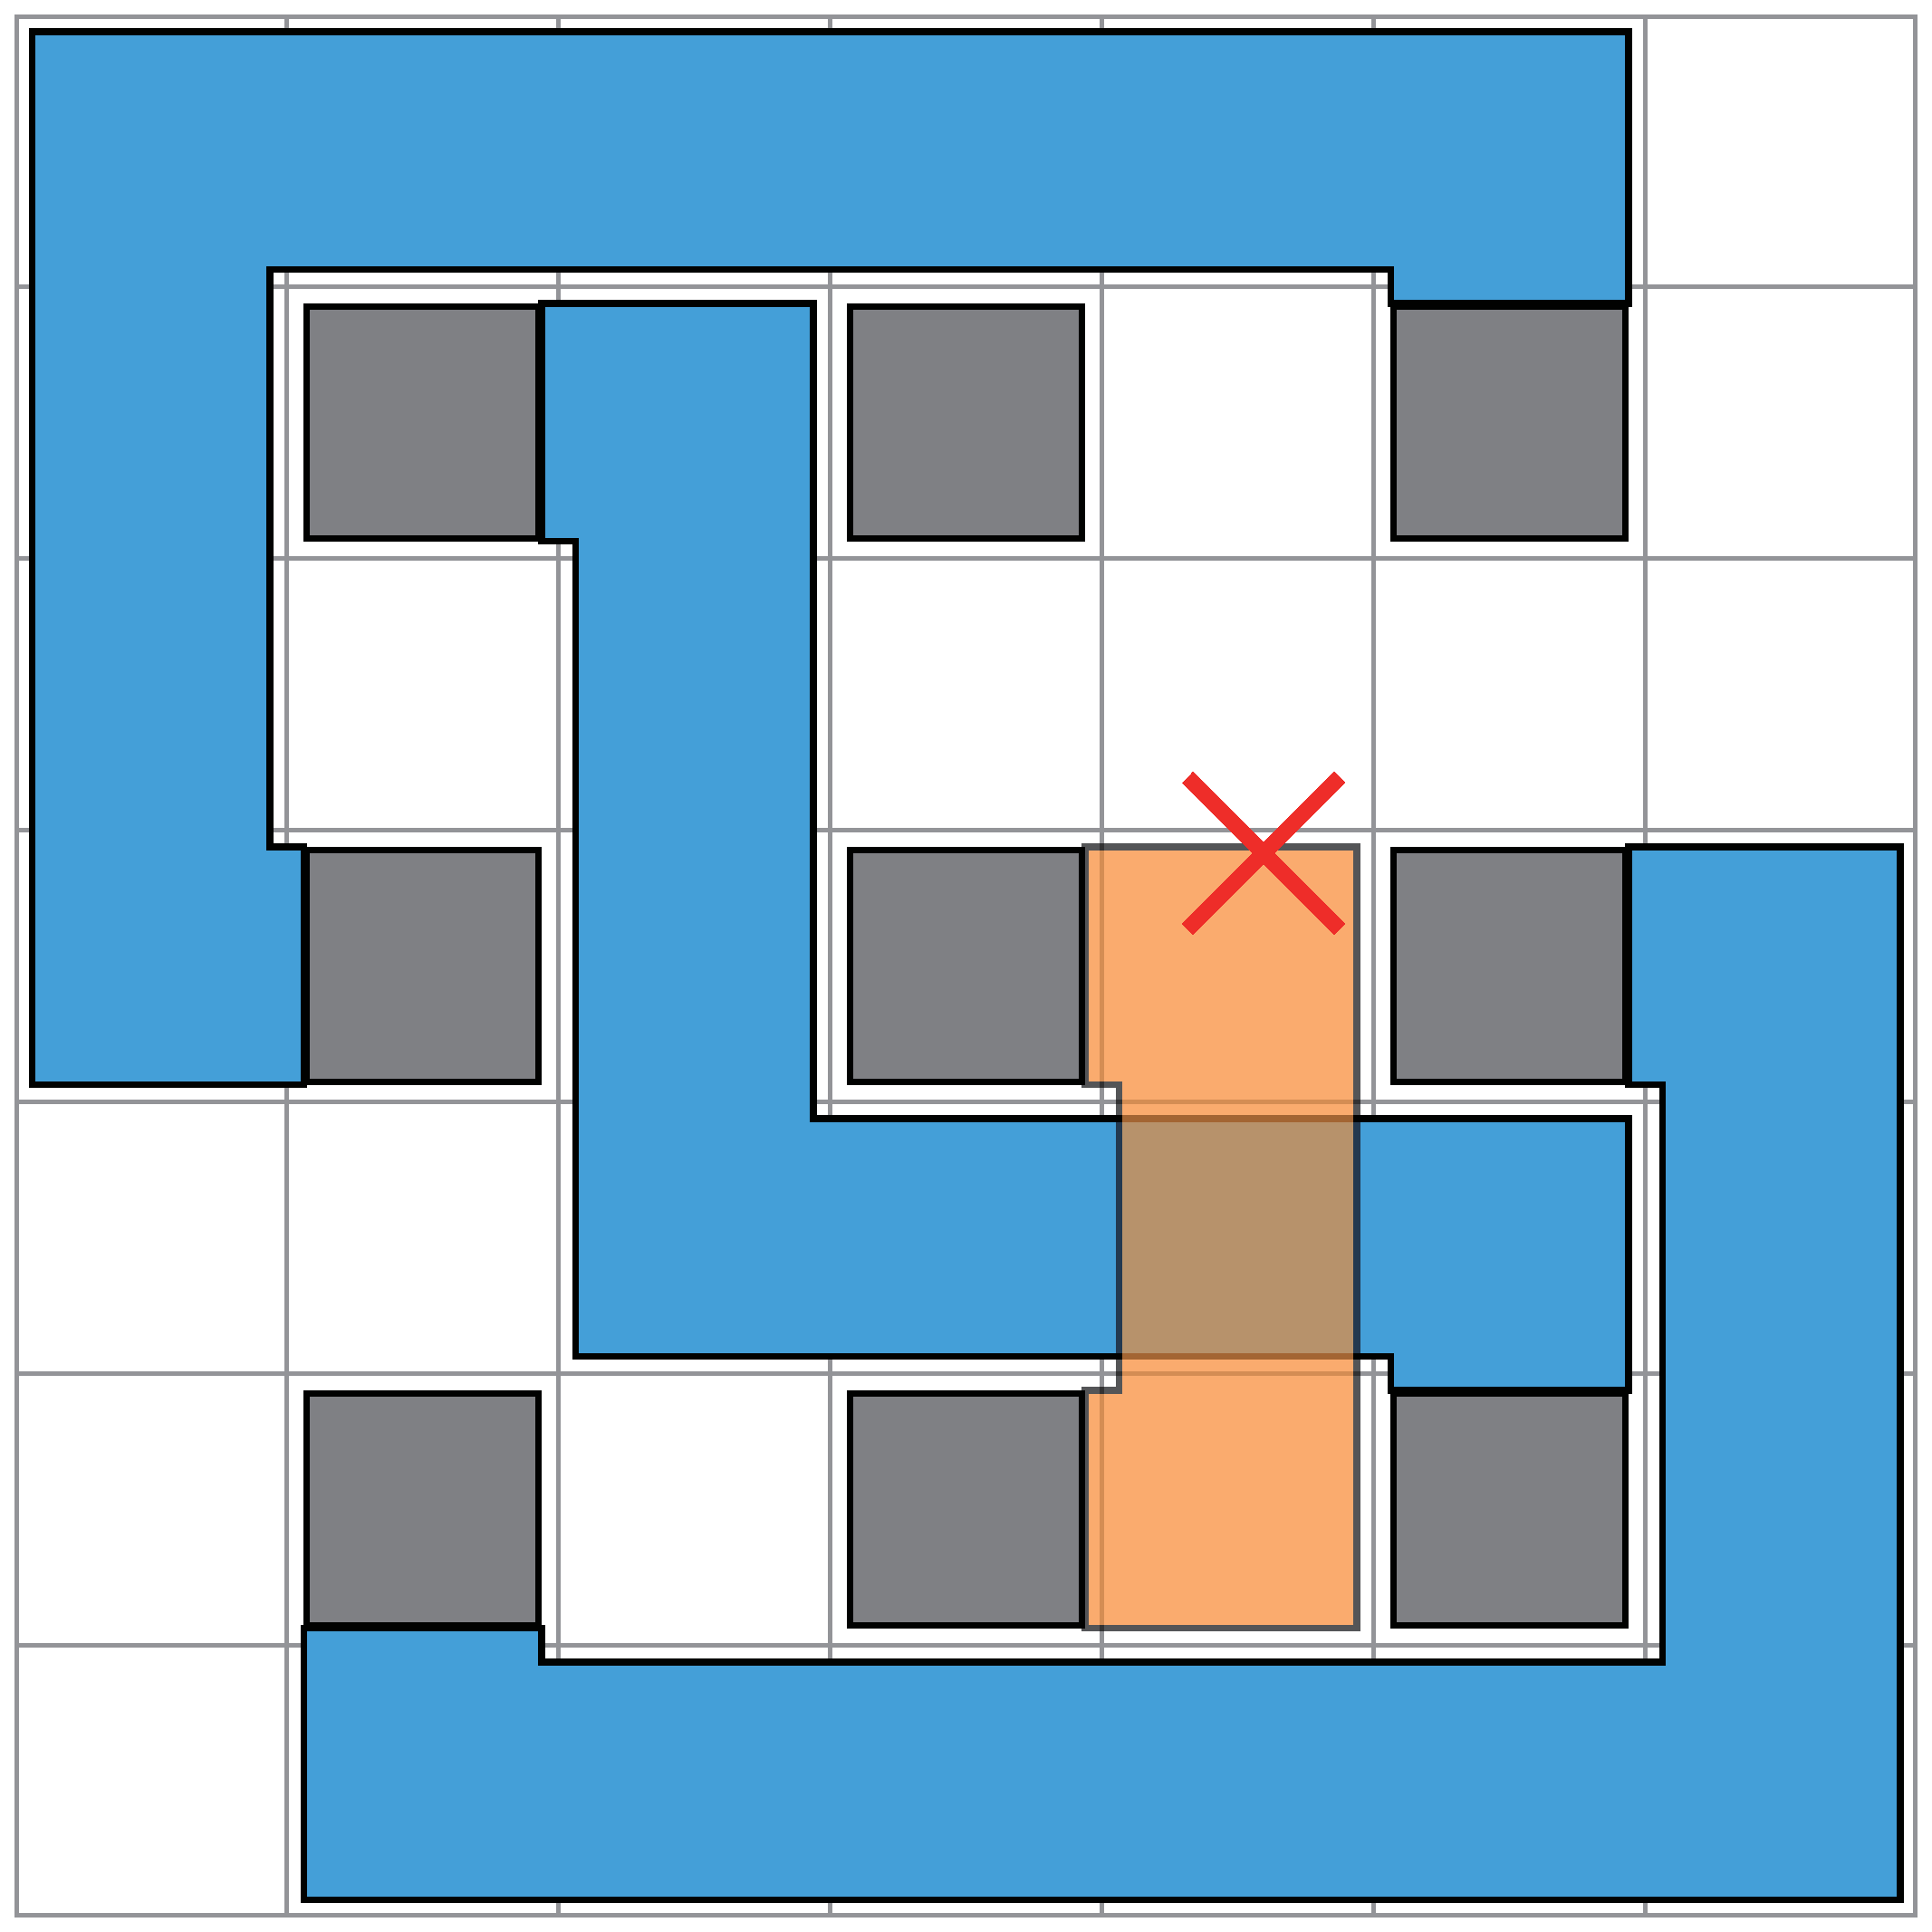
\includegraphics[scale=0.20]{figure/qubit_plane.eps}
            \vspace{0pt}\caption{}
            \label{qubit_plane}
            \vspace{-10pt}
        \end{figure}
        
    }

    \subsection{Pseudo Three-dimensional Surface Code}{
        \ \ \ First, we introduce the Surface Code implemented in the looped pipeline as described in Section~\ref{looped_pipeline}. In the looped pipeline architecture, we consider a single looped pipeline as a qubit in the Surface Code, as shown in Fig.~\ref{looped_pipeline_surface_code}. The red dashed lines represent a two-qubit gate for the two physical qubits in the looped pipeline. In the following description, the devices for measurement and initialization are not shown for simplicity.

        \begin{figure}[h]
            \centering
            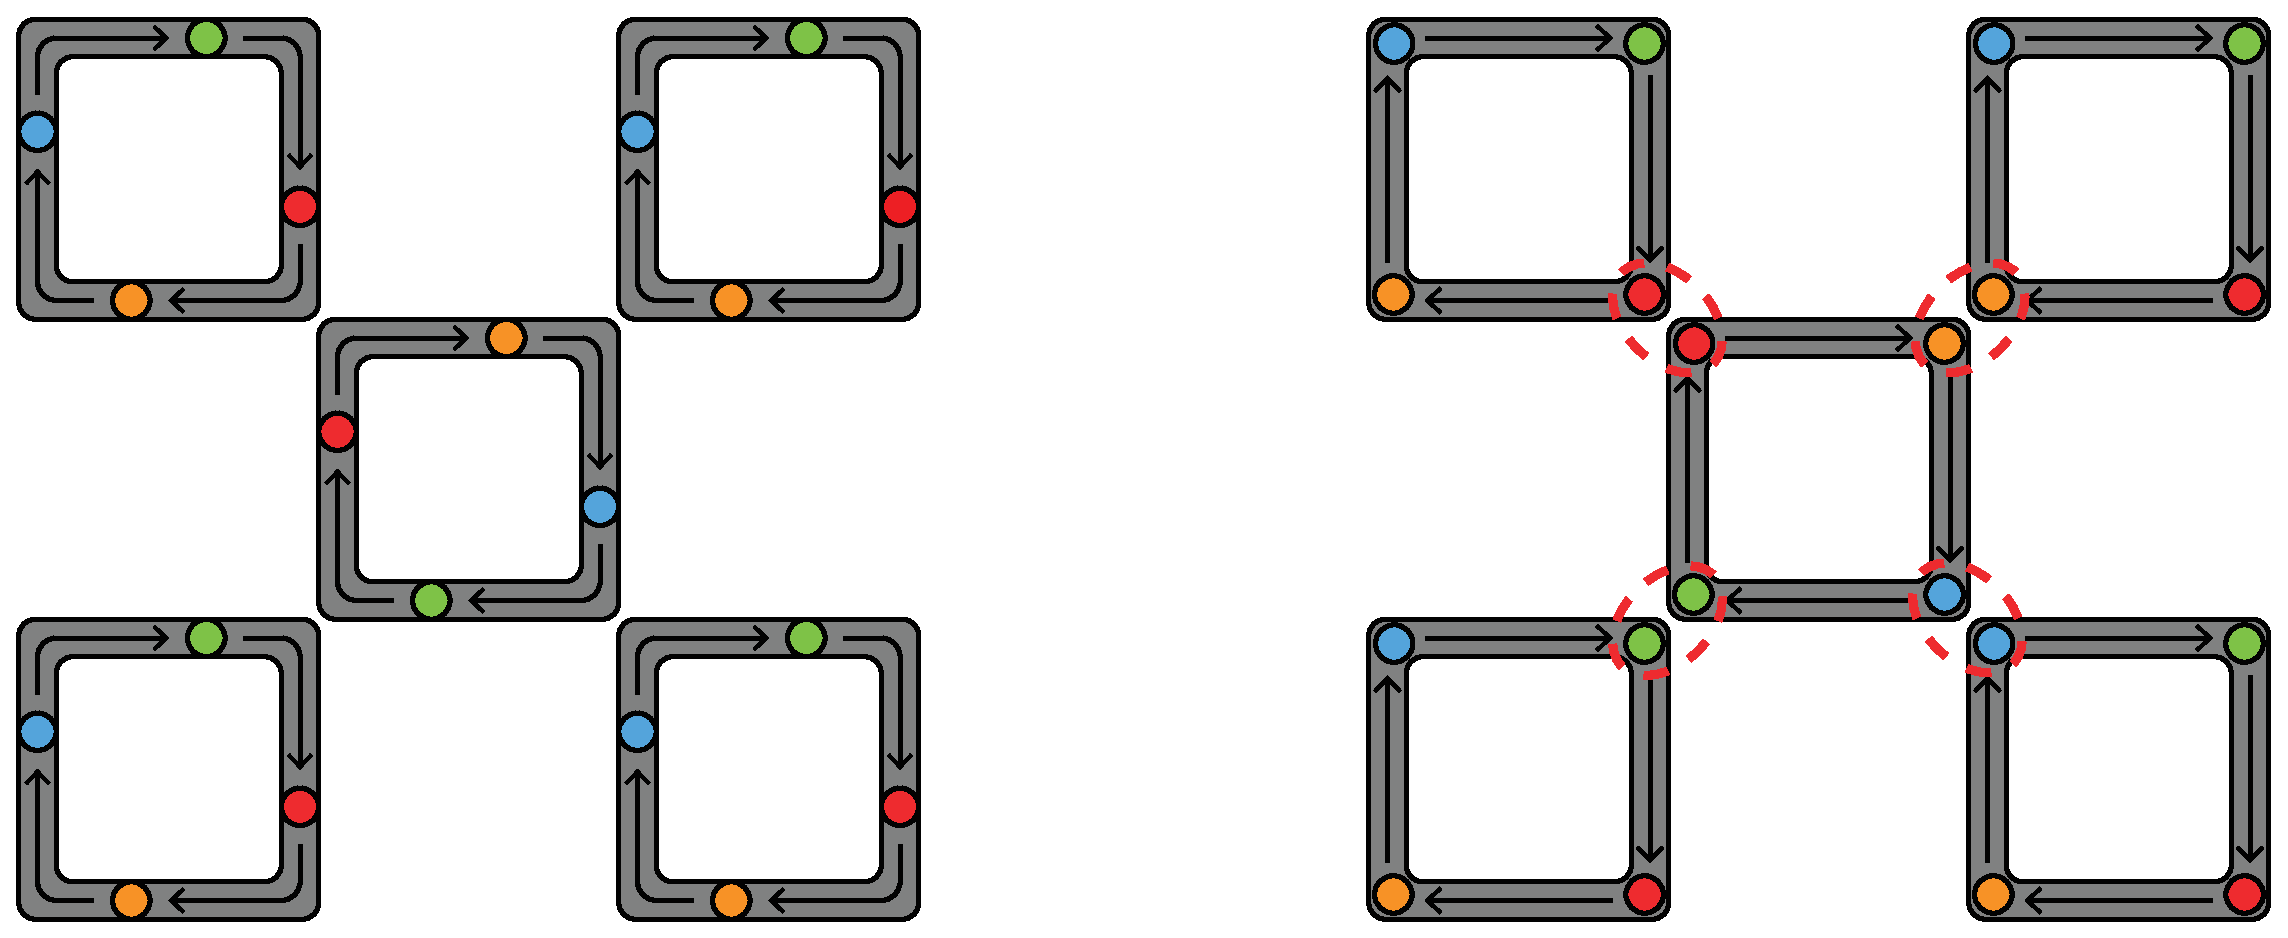
\includegraphics[scale=0.30]{figure/looped_pipeline_surface_code.eps}
            \vspace{0pt}\caption{}
            \label{looped_pipeline_surface_code}
            \vspace{-10pt}
        \end{figure}

        Considering the looped pipeline in the middle of the five pipelines as the ancilla qubit for syndrome measurement, and the looped pipelines surrounding the ancilla qubit as the data qubits, we can see that the allocation of looped pipelines corresponds to the Surface Code, as shown in Fig.~\ref{looped_pipeline_weak_surface_code}. There exist synchronized qubits with the same color in the looped pipeline.

        \clearpage
        \begin{figure}[h]
            \centering
            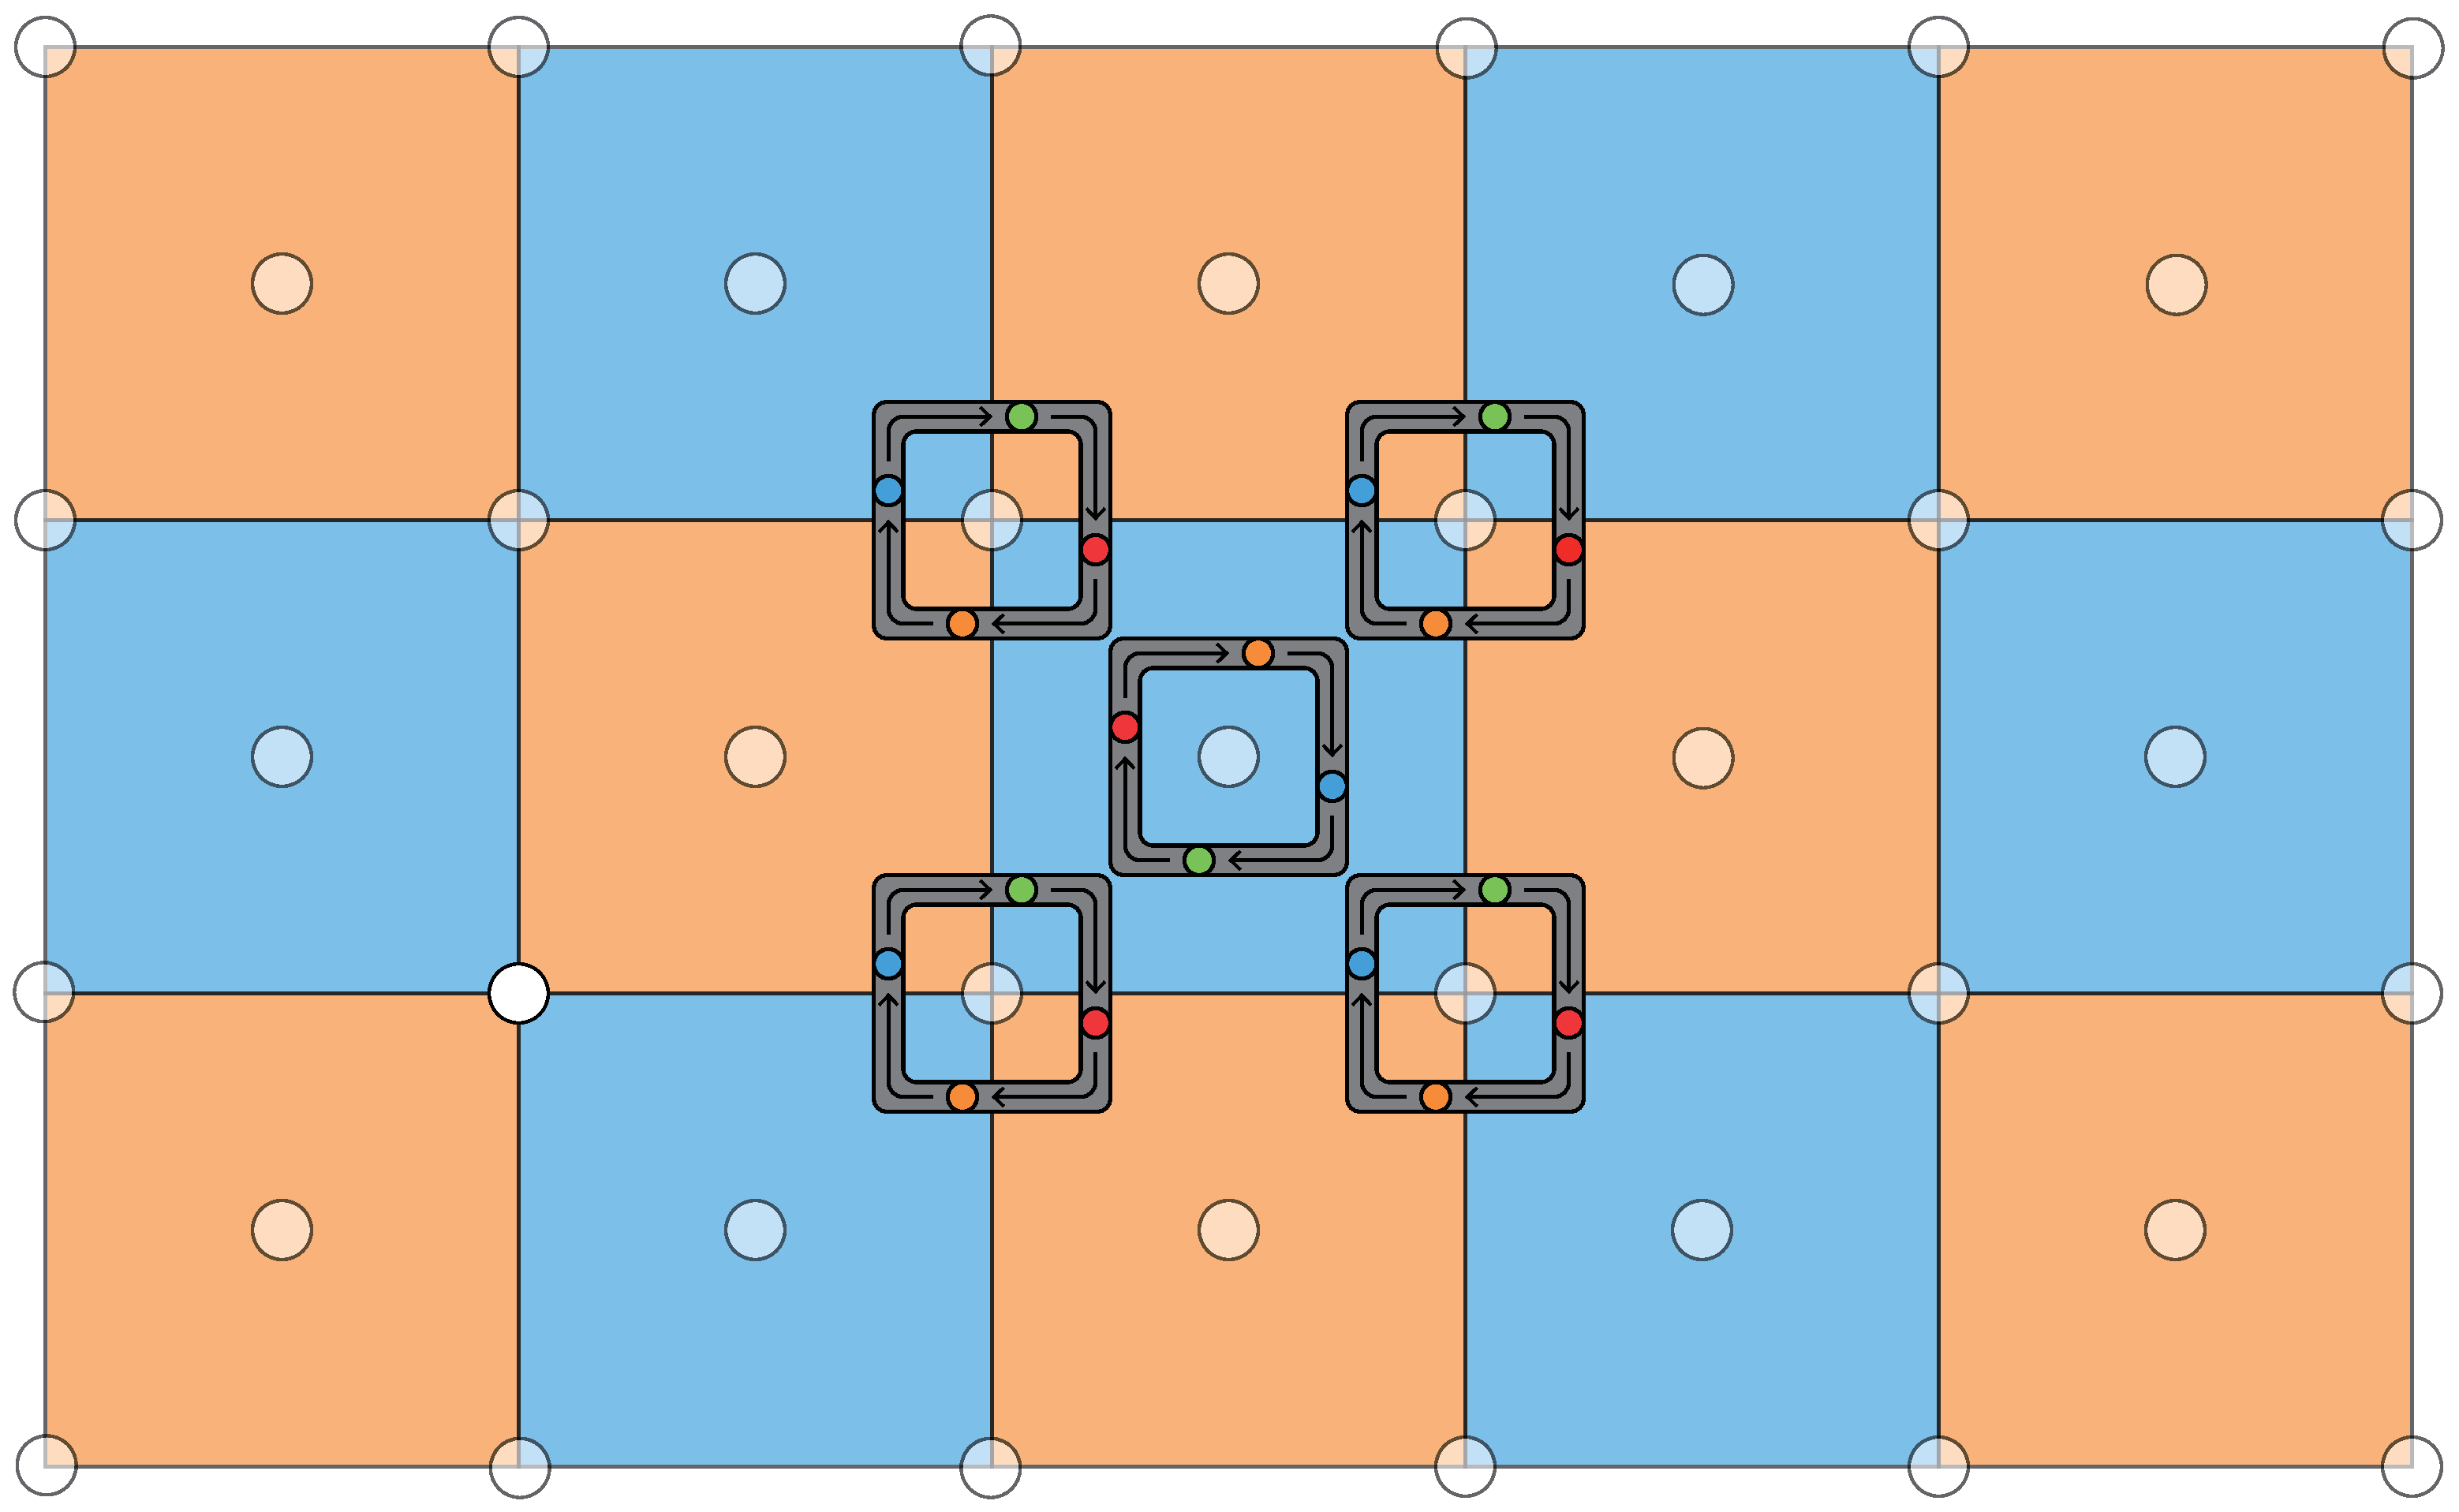
\includegraphics[scale=0.20]{figure/looped_pipeline_weak_surface_code.eps}
            \vspace{0pt}\caption{}
            \label{looped_pipeline_weak_surface_code}
            \vspace{-10pt}
        \end{figure} 

        In addition to the interloop interactions shown in the right half of Fig.~\ref{looped_pipeline_surface_code}, we can perform intraloop interactions as shown in Fig.~\ref{intraloop_interaction}.

        \begin{figure}[h]
            \centering
            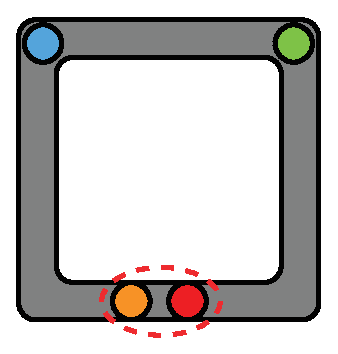
\includegraphics[scale=0.50]{figure/intraloop_interaction.eps}
            \vspace{0pt}\caption{}
            \label{intraloop_interaction}
            \vspace{-10pt}
        \end{figure}

        Now, we have four qubits in a single pipeline; thus, we have four stacks of Surface Codes, as shown in Fig.~\ref{stacked_surface_code}. In the following description, we refer to each stacked Surface Code as a "layer." Furthermore, when representing the pseudo-3D Surface Code as shown in Fig.~\ref{pipeline_to_surface}, we refer to each layer as a "floor." For example, we designate the red layer as floor 0 and the blue layer as floor 2. On the one hand, by introducing interloop interactions, as shown in Fig.~\ref{looped_pipeline_weak_surface_code}, we enable the construction of the Surface Code. On the other hand, by introducing intraloop interactions, we can perform logical two-qubit operations between qubits, each present in adjacent layers. Lastly, it is worth noting that in Fig.~\ref{pipeline_to_surface}, floor 0 and floor 3 are adjacent since the red qubits and orange qubits are adjacent in the looped pipelines.

        \begin{figure}[h]
            \centering
            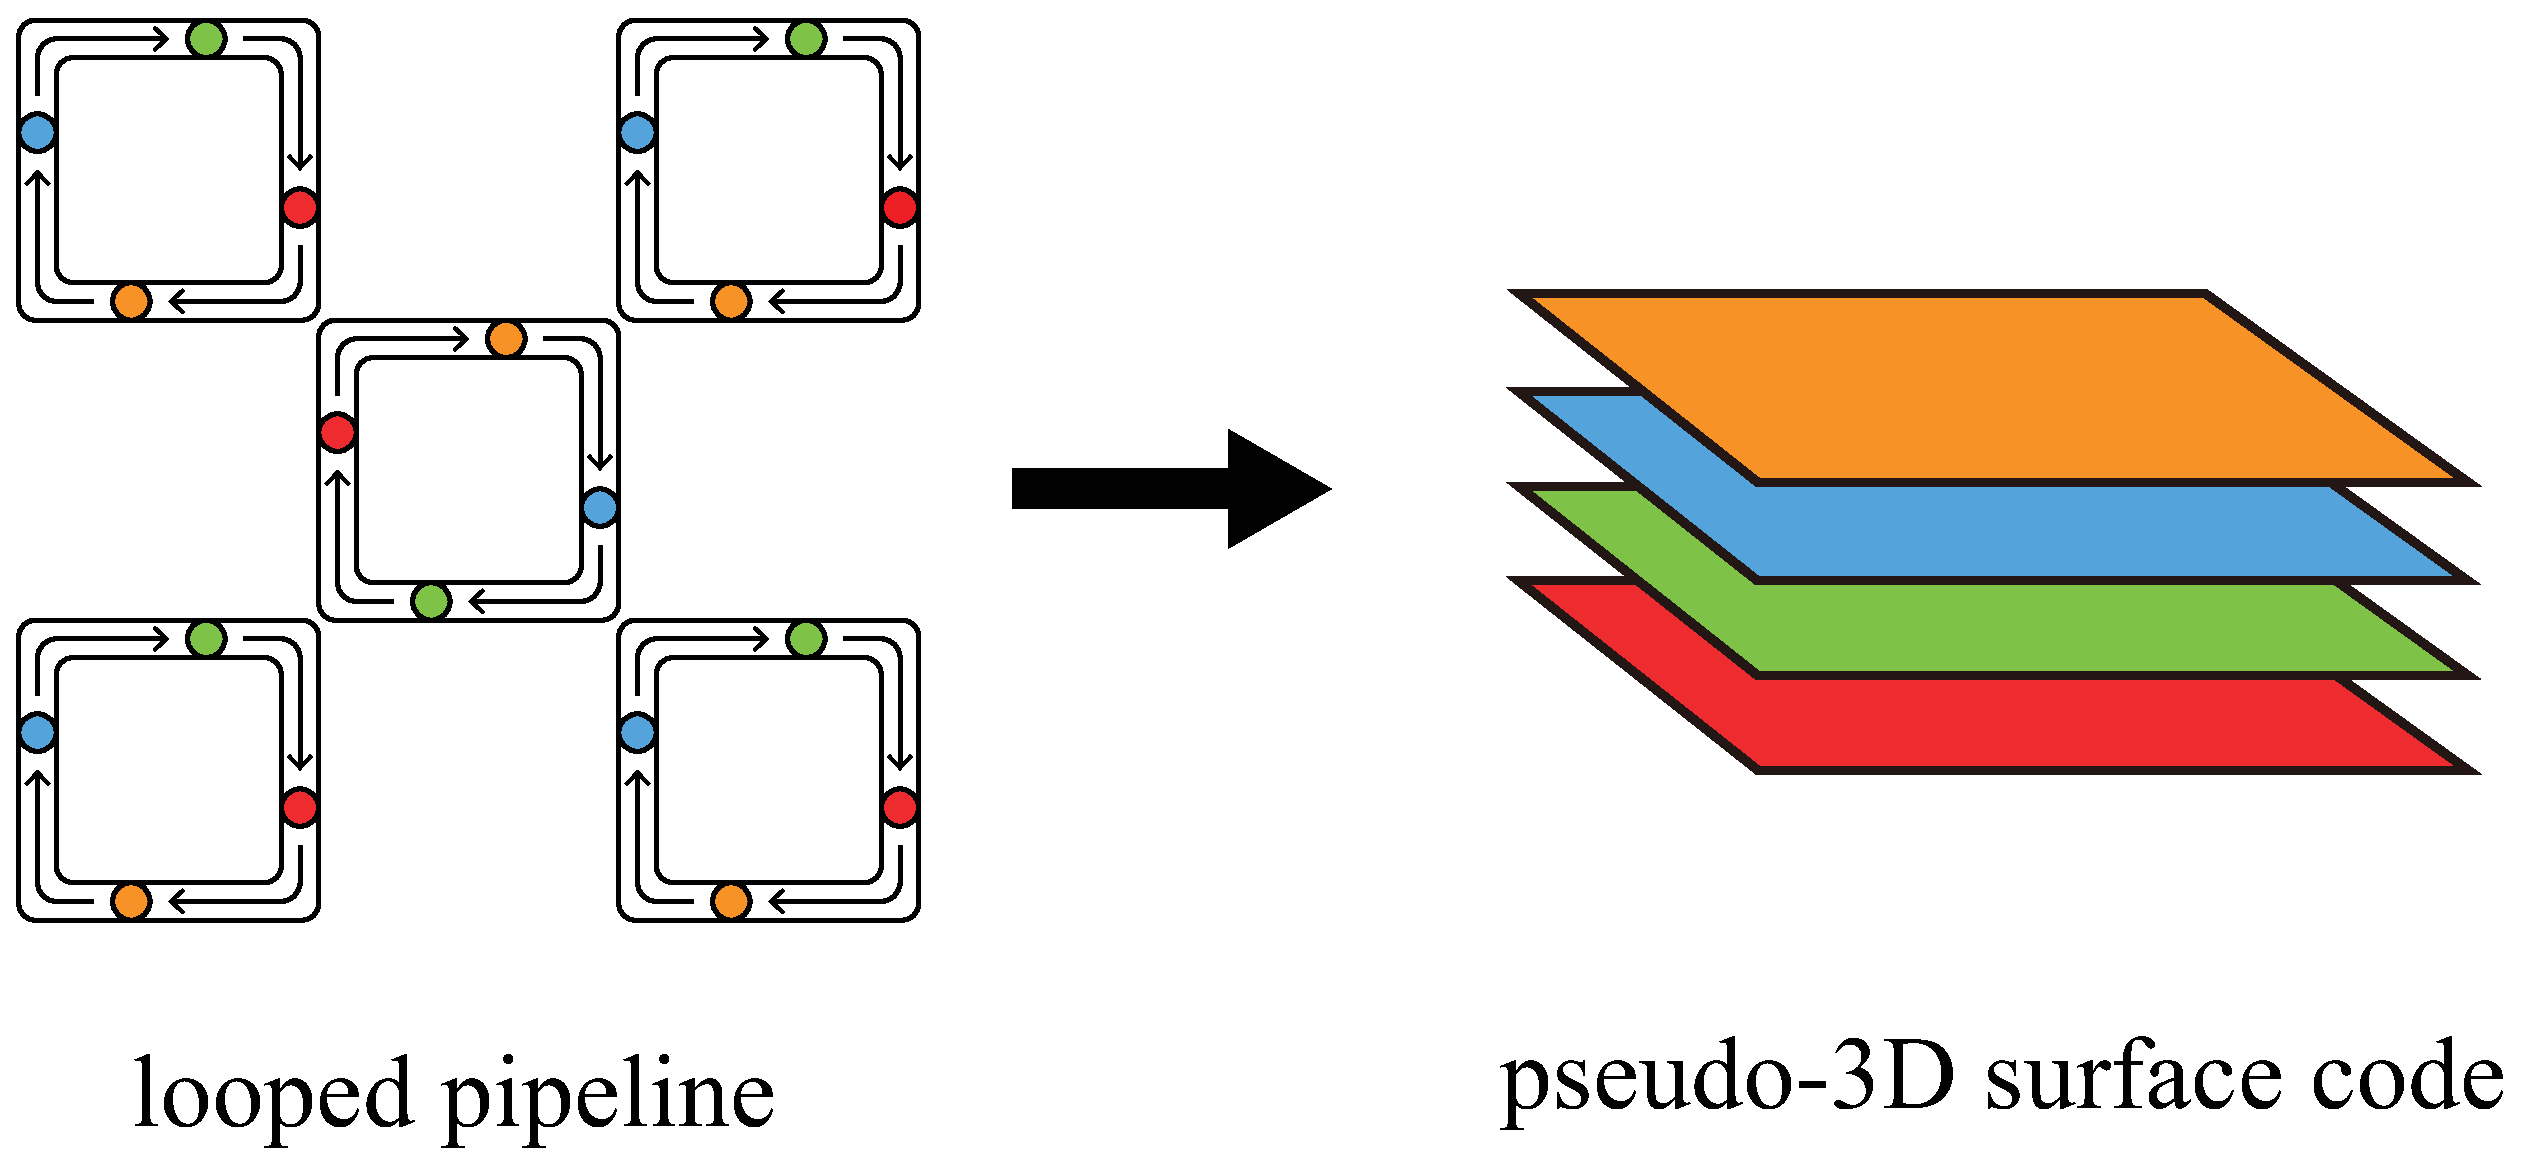
\includegraphics[scale=0.30]{figure/pipeline_to_surface.eps}
            \vspace{0pt}\caption{}
            \label{pipeline_to_surface}
            \vspace{-10pt}
        \end{figure}
        
    }

    \subsection{Lattice Surgery Routing}{
        \ \ \ In this subsection, we will show the advantage with using the psuedo-3D surface code for the lattice surgery routing. The numerical results are shown in Section.\ref{results}.\\
        \ \ \ In Fig.~\ref{3D_advantage_distance}, we are showing the distance advantage of the pseudo-3D Surface Code. When the blue operation in Fig.~\ref{3D_advantage_distance} is being processed, the orange operation needs to make a detour in the 2D Surface Code. However, in the pseudo-3D Surface Code, the orange operation can bypass the blue operation by utilizing the upper layer. Thus, the total cost for routing the blue and orange operations is less in the pseudo-3D Surface Code than in 2D.

        \begin{figure}[h]
            \centering
            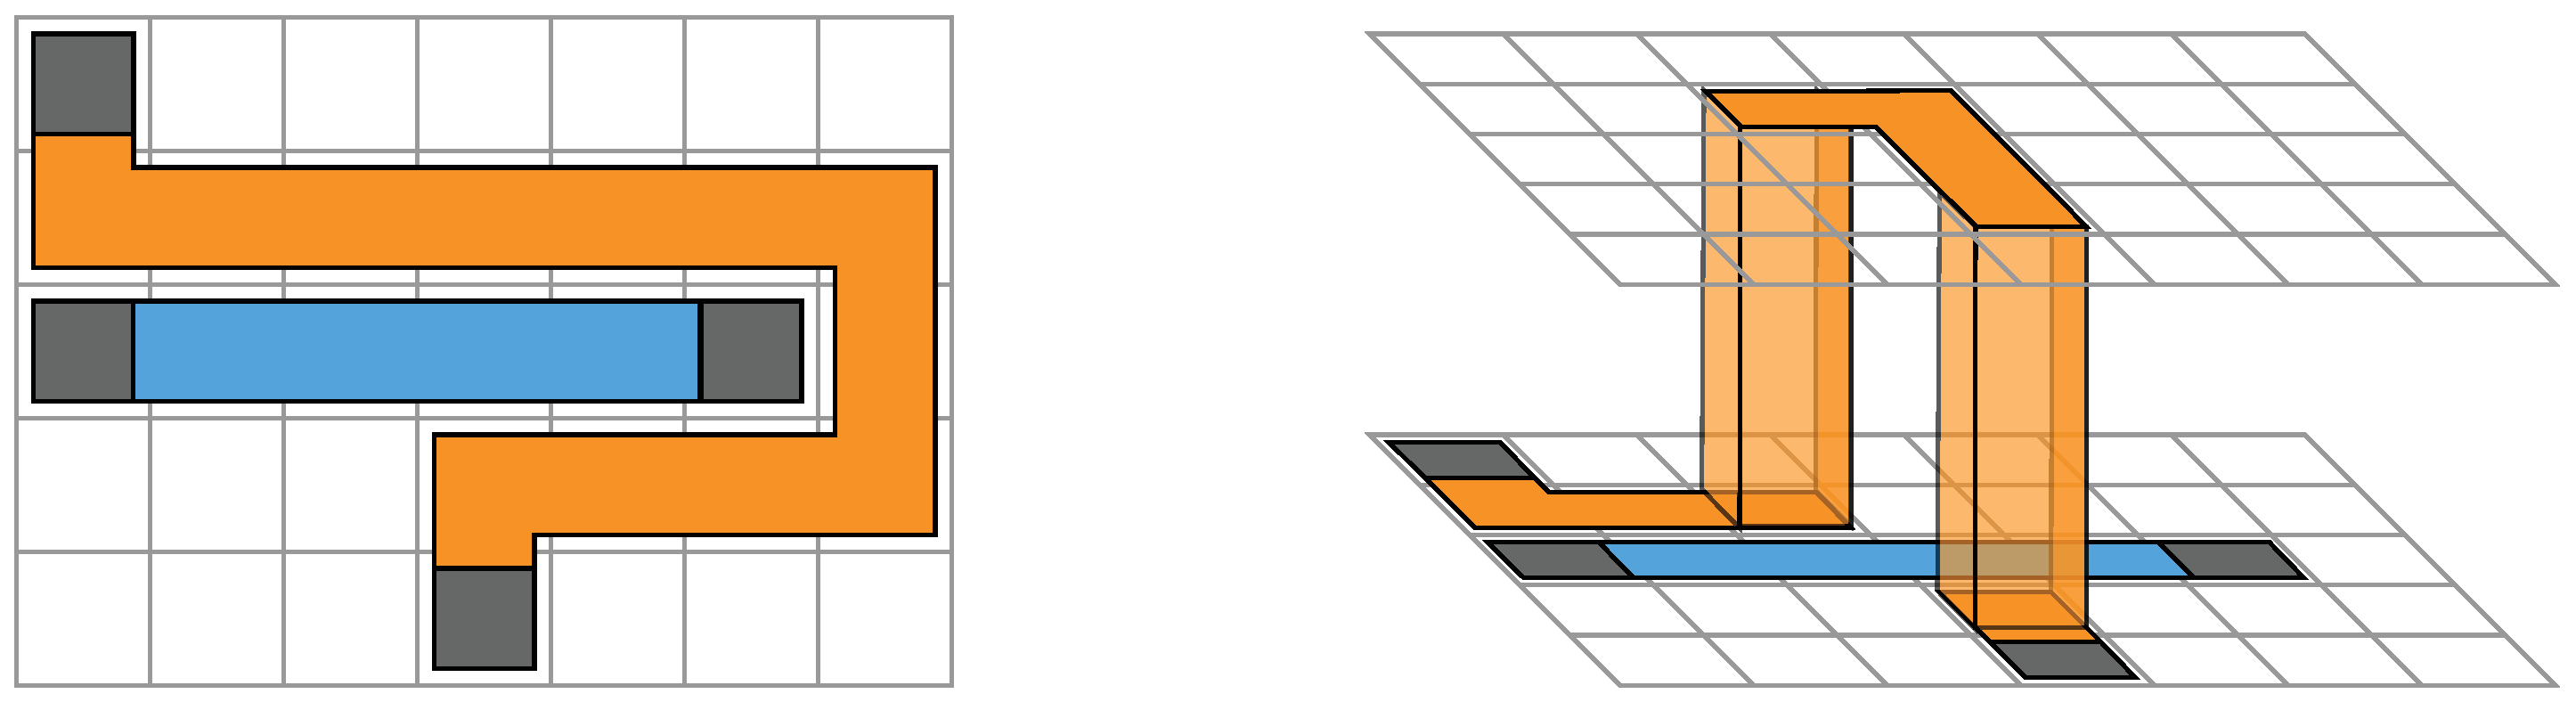
\includegraphics[scale=0.30]{figure/3D_advantage_distance.eps}
            \vspace{10pt}\caption{}
            \label{3D_advantage_distance}
            \vspace{-10pt}
        \end{figure}

        In Fig.~\ref{3D_advantage_parallel}, we are showing the parallelization advantage of the pseudo-3D Surface Code. When the blue operation in Fig.~\ref{3D_advantage_parallel} is being processed, the orange operation cannot be executed in the 2D Surface Code because there is no available route for the orange operation. However, in the pseudo-3D Surface Code, the orange operation can bypass the blue operation by utilizing the upper layer. Thus, the total time for executing the blue and orange operations is reduced in the pseudo-3D Surface Code compared to the 2D Surface Code.

        \begin{figure}[h]
            \centering
            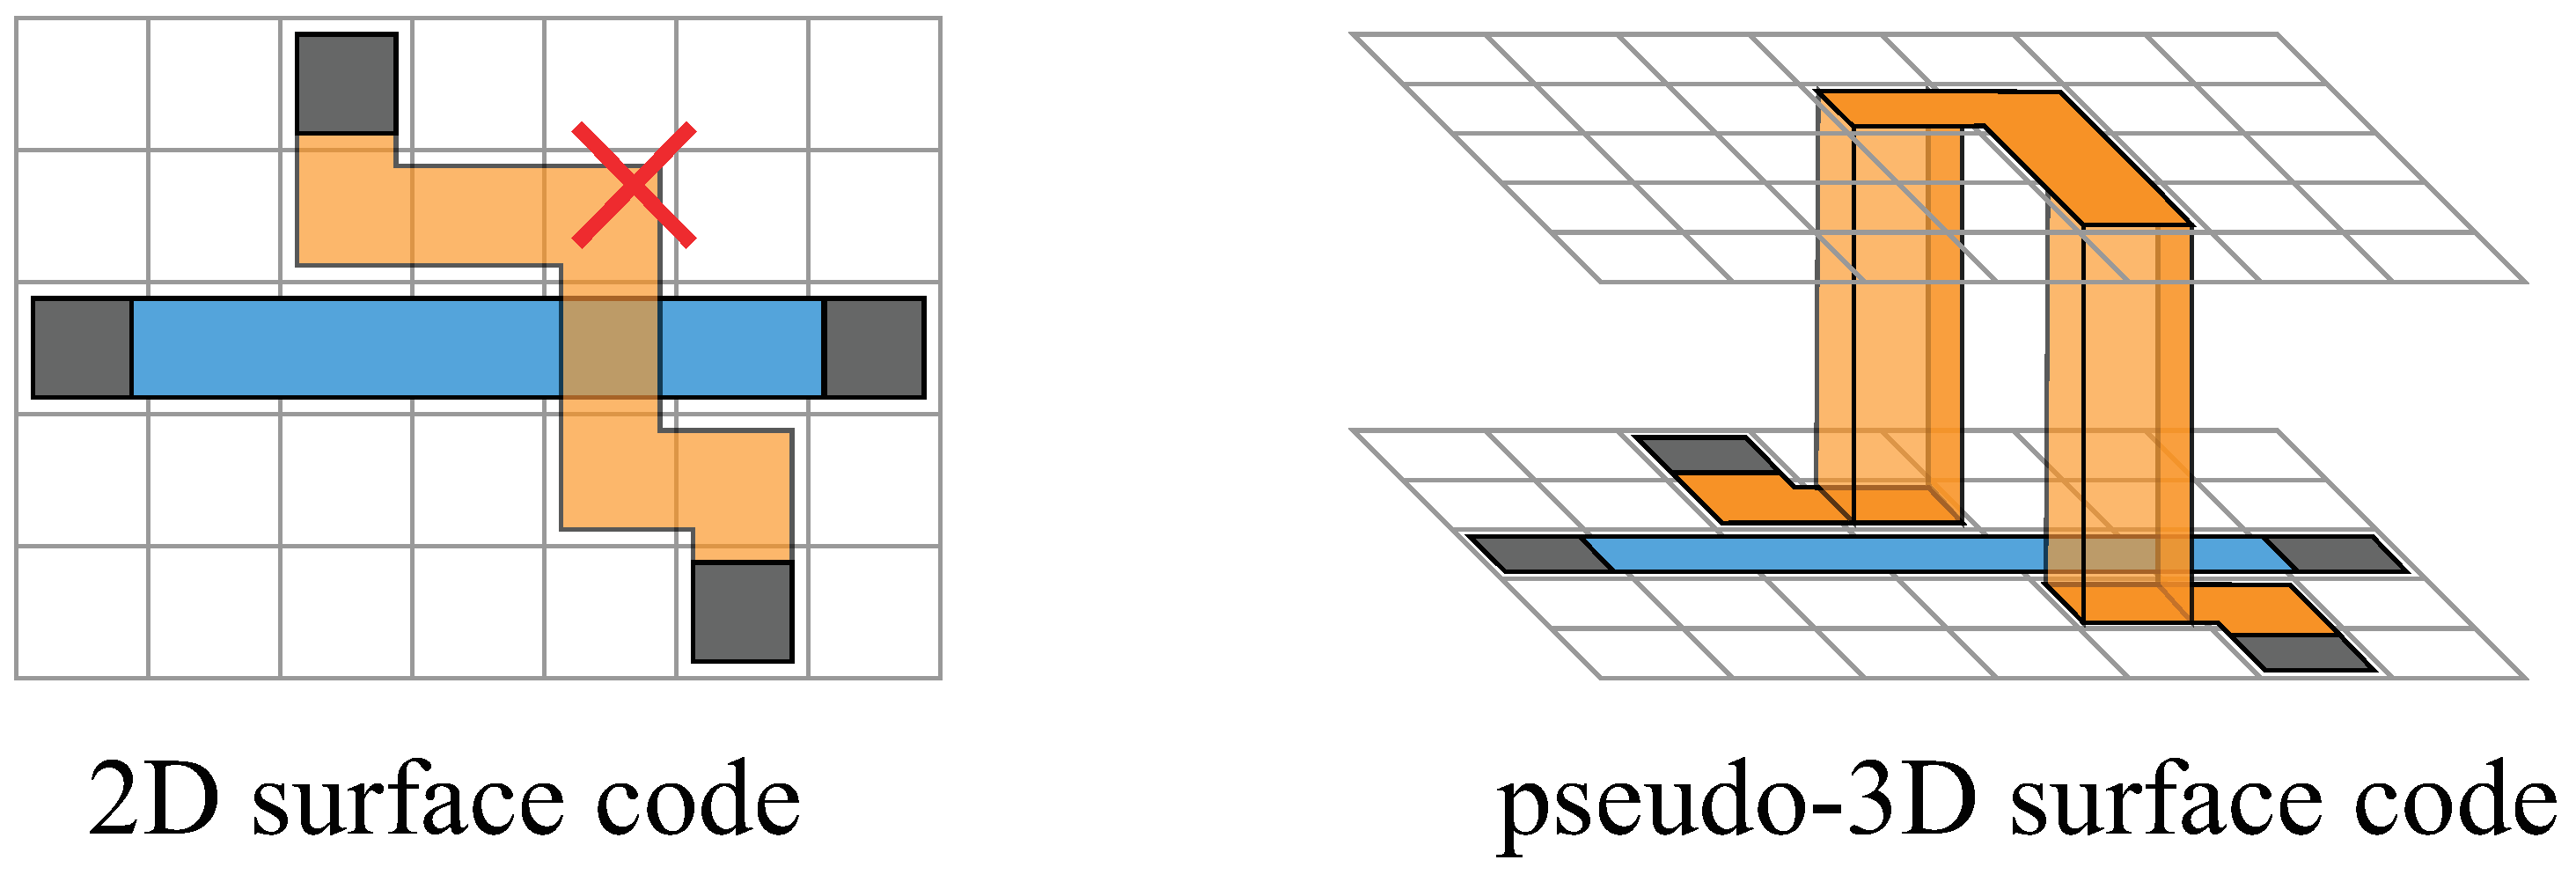
\includegraphics[scale=0.30]{figure/3D_advantage_parallel.eps}
            \vspace{10pt}\caption{}
            \label{3D_advantage_parallel}
            \vspace{-10pt}
        \end{figure}
    }
}
\end{document}